% uid: ""
% school: "college"
% level: "7eme"
% chapter: "التناظر المحوري"
% chapter_slug: "symetrie-axiale"
% title: "نقطة على المحور"
% difficulty: "Facile"
% tags: ["symetrie-axiale", "mediatrice", "point-sur-axe"]
% provenance: "own"
% batch: "2026-11-27-symetrie-axiale-7eme"
% Exercice 6/10 de la série 7ème « التناظر المحوري » (statement + \axsol + solution). Compiler avec XeLaTeX + axiomath.sty (+ axiomaths-logo.png).
\documentclass[12pt,a4paper]{article}
\usepackage[level=7b,color=0F766E]{axiomath}
\newcommand{\cm}{\,\mathrm{cm}}
\axsetup{title={التناظر المحوري}, corrige}

\begin{document}

\begin{corr}[title={نقطة على المحور}, stars=2, source={Axiomaths}]
$A'$ مناظرة النقطة $A$ بالنسبة إلى المستقيم $\Delta$ حيث $AA'=6\cm$. المستقيم $(AA')$ يقطع $\Delta$ في $H$.
\begin{center}
\begin{tikzpicture}[scale=0.6]
  \draw[very thick] (0,-3.8)--(0,3.8) node[above] {$\Delta$};
  \draw[thick] (-3,1)--(3,1);
  \fill (-3,1) circle (2.5pt) node[left] {$A$};
  \fill (3,1) circle (2.5pt) node[right] {$A'$};
  \fill (0,1) circle (2.5pt) node[below right] {$H$};
\end{tikzpicture}
\end{center}
\begin{enumerate}
  \item احسب $AH$ ، ثم حدّد قيس الزاوية التي يكوّنها $(AA')$ مع $\Delta$.
  \item $M$ نقطة من $\Delta$ حيث $MA=3{,}5\cm$. ما هي مناظرة $M$ بالنسبة إلى $\Delta$ ؟ استنتج $MA'$.
  \item $N$ نقطة حيث $NA=NA'=5\cm$. بين أن $N$ تنتمي إلى $\Delta$.
\end{enumerate}
\axsol
\begin{enumerate}[itemsep=14pt]
  \item\leavevmode
  \begin{prop}[تعريف]
  $A'$ مناظرة $A$ بالنسبة إلى $\Delta$ معناه : $\Delta$ هو محور $[AA']$ ، أي \ib{$\Delta\perp(AA')$ في منتصف $[AA']$}.
  \end{prop}
  $H$ هي نقطة تقاطع $(AA')$ و $\Delta$ ، فهي منتصف $[AA']$ :
  \[AH=\dfrac{AA'}{2}=\dfrac{6}{2}=3\cm\]
  و $(AA')\perp\Delta$ : الزاوية قائمة، قيسها \ib{$90^\circ$}.
  \item $M$ تنتمي إلى $\Delta$ ، إذن \ib{مناظرتها هي $M$ نفسها}.

  التناظر يحوّل $M$ إلى $M$ و $A$ إلى $A'$ ، فيحوّل القطعة $[MA]$ إلى $[MA']$. والتناظر يحافظ على الأطوال :
  \[MA'=MA=3{,}5\cm\]
  \item\leavevmode
  \begin{prop}[محور قطعة]
  كل نقطة \ib{متساوية البعد} عن طرفي قطعة تنتمي إلى \ib{محور هذه القطعة}.
  \end{prop}
  $NA=NA'=5\cm$ ، إذن $N$ تنتمي إلى محور $[AA']$.

  ومحور $[AA']$ هو $\Delta$ ، إذن \ib{$N\in\Delta$}.
  \begin{center}
  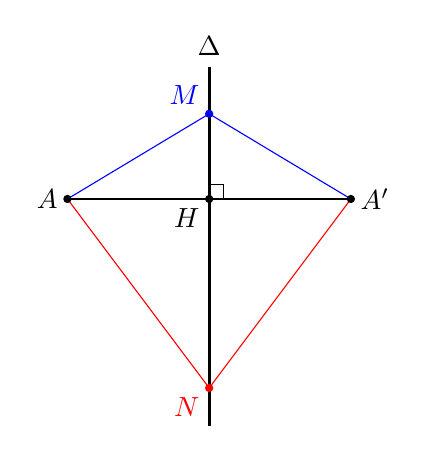
\begin{tikzpicture}[scale=0.6]
    \draw[very thick] (0,-3.8)--(0,3.8) node[above] {$\Delta$};
    \draw[thick] (-3,1)--(3,1);
    \draw (0,1.3)--(0.3,1.3)--(0.3,1);
    \draw[blue] (-3,1)--(0,2.803)--(3,1);
    \draw[red] (-3,1)--(0,-3)--(3,1);
    \fill (-3,1) circle (2.5pt) node[left] {$A$};
    \fill (3,1) circle (2.5pt) node[right] {$A'$};
    \fill (0,1) circle (2.5pt) node[below left] {$H$};
    \fill[blue] (0,2.803) circle (2.5pt) node[above left] {$M$};
    \fill[red] (0,-3) circle (2.5pt) node[below left] {$N$};
  \end{tikzpicture}
  \end{center}
\end{enumerate}
\end{corr}

\end{document}
